\documentclass[letterpaper,10pt]{article}
\usepackage[margin=2cm]{geometry}

\usepackage{graphicx}
\usepackage{amsmath}
\usepackage{amsfonts}
\usepackage{amssymb}
\usepackage[colorlinks]{hyperref}

\newcommand{\panhline}{\begin{center}\rule{\textwidth}{1pt}\end{center}}

\setlength{\parindent}{0em}
\setlength{\parskip}{0.2em}

\title{\textbf{01 Introduction}}
\author{Pradeep Ravikumar(Lecturer), HMW-Alexander(Noter)}

\begin{document}

\maketitle

\panhline
\href{../index.html}{Back to Index}

\panhline
\tableofcontents

\section*{Resources}

\begin{itemize}
	\item \href{../../Lectures/01_Introduction.pdf}{Lecture}
	\item \href{../../Books/Pattern_Recognition_And_Machine_Learning.pdf}{Textbook}
\end{itemize}

\panhline

\section{Info}

\subsection{Final Project}

Kaggle style data analysis project, with leaderboard.

What is Kaggle\footnote{\url{https://en.wikipedia.org/wiki/Kaggle}}?
\begin{itemize}
	\item In 2010, Kaggle was founded as a platform for predictive modelling and analytics competitions on which companies and researchers post their data, and statisticians and dta miners from all over the world compete to produce the best models.
	\item In April 2015, Kaggle released the first version of their \textbf{Scripte}\footnote{\url{https://www.kaggle.com/kernels}} product onto their platform. Scripts allows users to write, run, and publicly share their code on Kaggle. On 8 July 2016, Kaggle renamed its \textbf{Scripts} product to \textbf{Kernels}.
	\item In January 2016, Kaggle released their \textbf{Datasets}\footnote{\url{https://www.kaggle.com/datasets}} product, making a selection of public datasets available on Kaggle.
\end{itemize}

\section{What is Machine Learning?}

\textbf{Algorithms} that improve their \textbf{knowledge} towards some task with \textbf{data}.
\begin{figure}[!h]
	\centering
	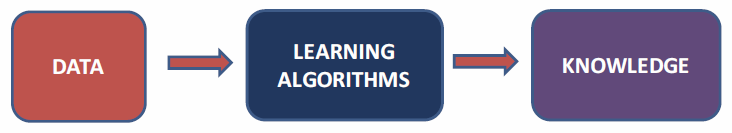
\includegraphics[width=15cm]{./img/machinelearning.png}
\end{figure}

\subsection{Different Goals with Different Fields}

\begin{itemize}
	\item Machine Learning: the underlying mechanisms and algorithms that allow improving our knowledge with more data.
	\item Statistics: the understanding of the data at hand.
	\item Artificial Intelligence: build an intelligent agent.
	\item Data Mining: to extract patterns from large-scale data
	\item Data Science: the science encompassing collection, analysis, and interpretation of data.
\end{itemize}

\section{Three axes of ML}

\begin{itemize}
	\item Data
	\item Tasks
	\item Algorithms
\end{itemize}

\subsection{Data}

\begin{itemize}
	\item Fully observed
	\item Partially observed
	\begin{itemize}
		\item systematically not observed.
		\item missing some of the time.
	\end{itemize}
	\item Actively collect/sense data.
\end{itemize}

\subsection{Algorithms}

\begin{itemize}
	\item Model-based methods
	\begin{itemize}
		\item Probabilistic model of the data
		\item Parametric models
		\item Nonparametric models
	\end{itemize}
	\item Model-free methods
\end{itemize}

\subsubsection{Model-based ML}

\begin{figure}[!h]
	\centering
	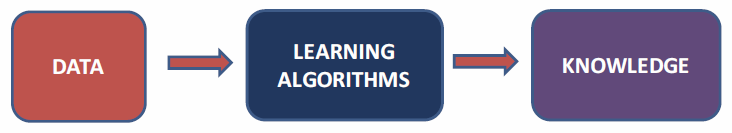
\includegraphics[width=15cm]{./img/machinelearning.png}\\
	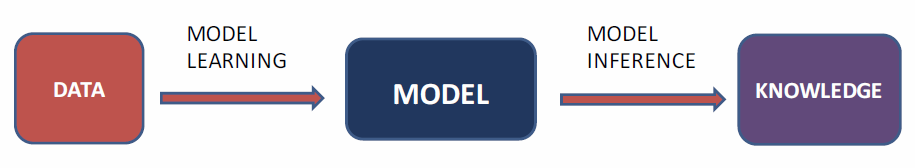
\includegraphics[width=15cm]{./img/modelbasedml.png}
\end{figure}

Learning and Inference
\begin{itemize}
	\item Learning: from data to model
	\begin{itemize}
		\item A model thus is a summary of the data, and also a story of how the data was generated.
		\item Could thus be used to describe how future data can be generated.
	\end{itemize}
	\item Inference: from model to knowledge
	\begin{itemize}
		\item given the model, what can we answer to the questions.
	\end{itemize}
\end{itemize}

Parametric and Nonparametric
\begin{itemize}
	\item Parametric models
	\begin{itemize}
		\item Fixed-size models that do not grow with the data.
		\item More data $\Rightarrow$ fit the model better.
		\item Model: data = point on line + noise
	\end{itemize}
	\item Nonparametric models
	\begin{itemize}
		\item Models that grow with the data.
		\item More data $\Rightarrow$ more complex model.
		\item Model: data = point on smooth curve + noise
	\end{itemize}
\end{itemize}

\subsubsection{Model-free ML}

No modeling assumption.

\subsection{Knowledge/Tasks}

\begin{itemize}
	\item Prediction: estimate output given input
	$$\text{given } X\in \text{ feature space } \mathcal{X} \text{, predict } Y\in \text{ label space } \mathcal{Y}$$
	\begin{itemize}
		\item Classification: discrete labels
		\item Regression: continuous labels
	\end{itemize}
	\item Description (also called unsupervised learning)
	$$\text{Given }X\in\text{ feature space }\mathcal{X}\text{, learn }f(X) $$
	\item E.g.
	\begin{itemize}
		\item Density estimation
		\item Clustering
		\item Dimensionality reduction
	\end{itemize}
\end{itemize}

\section{Machine Learning Subfields}

\begin{itemize}
	\item Supervised learning
	\begin{itemize}
		\item Data consists of both inputs and outputs
		\item Tasks consists of prediction
	\end{itemize}
	\item Semi-supervised learning
	\begin{itemize}
		\item Data consist of inputs and only some of them with outputs
		\item Tasks consists of prediction
	\end{itemize}
	\item Reinforcement learning
	\begin{itemize}
		\item Data consists of rewards that come through taking \textbf{actions} that has a feedback
		\item Task: maximize reward.
	\end{itemize}
	\item Multi-agent systems
	\begin{itemize}
		\item multiple agents with same setup as in reinforcement learning.
		\item the data also consists of other agents' actions.
	\end{itemize}
\end{itemize}

\end{document}



